\documentclass[a4paper]{report}
\usepackage[utf8]{inputenc}
\usepackage[german]{babel}
\usepackage{graphicx}
\usepackage[font]{}

\begin{document}

\chapter{Einführung}

Die  vier Wirtschaft Subjekten:
\newline
\newline
\newline
\newline
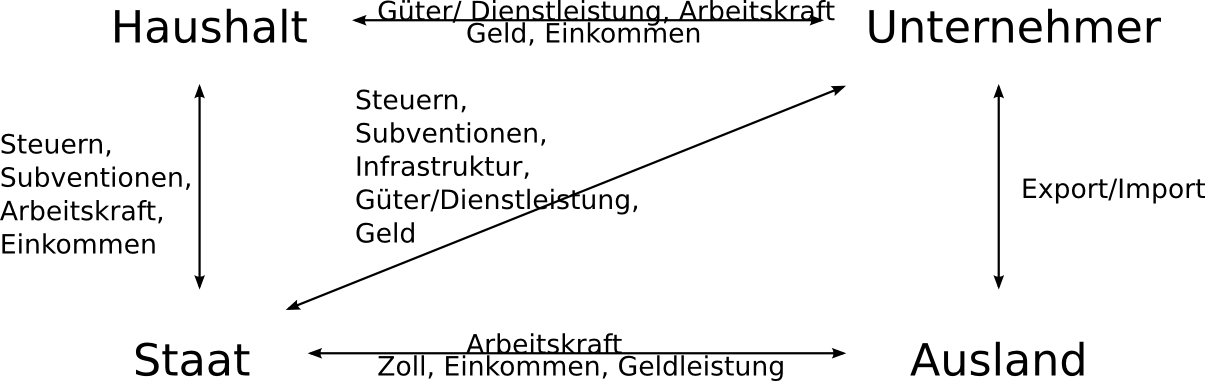
\includegraphics[scale=0.8]{image/image1.png}
\newline
\newline
\newline
\newline
Die Wirtschaftstätigkeit eines Landes wird zahlenmäßig erfasst, wobei verschiedene Ströme festgestellt werden. Zwischen den vier Wirtschaft Subjekten kommt es zu Transaktionen, Austausch von Gütern. Es gibt zwei gegenläufige Ströme:

\begin{itemize}
\item Realer Strom: Güter (Waren) und Dienstleistung
\item Monetärer Strom: Geld (Geldstrom)
\end{itemize}

Am Geldstrom wird das Volkseinkommen gemessen, am Güterstrom das Sozialprodukt. Das Sozialprodukt ist ein genereller Maßstab für die Wirtschaftskraft eines Landes. Je größer es ist, desto mehr kann im Allgemeinem verbraucht werden und desto größer ist der rechnerischer Wohlstand der Bevölkerung so fern dieser einigermaßen gleich verteilt ist.

\chapter{Güter}

Einteilung der Güter nach der Verfügbarkeit:

\begin{itemize}
\item öffentliche Güter (unbegrenzt vorhanden)
\item knappe Güter (Sachgüter, Dienstleistung, Rechte, Eigentumsrecht, ...)
\end{itemize}

Einteilung der Güter nach Verwendung:

\begin{itemize}
\item Konsumgüter
	\begin{itemize}
	\item Verbrauchsgüter (für einmaligen Gebrauch z.B. Nahrung, ...)
	\item Gebrauchsgüter (für mehrmaligen Gebrauch z.B. Auto, ...)
	\end{itemize}
\item Produktionsgüter (Güter mit den sich andere Güter herstellen lassen können)
\end{itemize}

\chapter{Produktionsfaktoren}

\section{Produktionsfaktoren}

\begin{itemize}
\item Boden
\item Arbeit
\item Wissen (Know-How)
\item Boden
\end{itemize}




\chapter{Taylorismus}

Wenn man einen komplexen Arbeitsprozess in möglichst viele kleinere Prozesse zerteilt, spricht man von Taylorismus. Zudem trennt man räumlich und personell die ausführende Arbeit mit der dispositiven Arbeit (Weisungsbefugnis).

\section{Vor- und Nachteile:}

\subsection{Vorteile:}

\begin{itemize}
\item Arbeiter benötigen nicht spezielles Wissen (billige Arbeitskräfte) oder lange Einarbeitungsphase
\item Arbeiter können leicht ersetzen werden
\item Transparenz in der Produktion und auch leichte Fehlersuche im Arbeitsprozess
\end{itemize}

\subsection{Nachteile:}

\begin{itemize}
\item Arbeiter langweilen sich, Monotonie $\rightarrow$ keine Motivation (kann zu Streiks führen)
\item körperliche Schäden $\rightarrow$ einseitige Belastung (z.B. Räder stemmen)
\item schlechtes Arbeitsklima, da es zu keiner Kommunikation zwischen den Arbeitern möglich ist
\item sinkende Lern- und Anpassungsmöglichkeiten an neue Aufgaben
\end{itemize}

\section{Andere Arbeitsformen}

\begin{itemize}
\item job rotation: Nach einem festen System werden regelmäßig die Arbeitsplätze getauscht. Die Struktur der Aufgaben wird nicht angerührt.
\item job enlargement: Zusätzliche Aufgaben werden zusammengeführt.
\item job enrichment: qualitative Ausweitung der Aufgaben, Eigenverantwortung
\item Team Arbeit (Projekt): große Motivation
\end{itemize}

\chapter{Wirtschaftssektoren}

\begin{itemize}
\item primärer Wirtschaftssektor: Urgewinnung
\item sekundärer Wirtschaftssektor: Produktion
\item tertiärer Wirtschaftssektor: Dienstleistung
\item quartärer Wirtschaftssektor: IT
\end{itemize}

\chapter{Arbeitslosigkeit}

\section{Definition}

Eine Person ist dann Arbeitslos, wenn die Person arbeitsfähig und arbeitswillig ist, sie schon einmal gearbeitet hat und nach Arbeit sucht.

\section{Arten der Arbeitslosigkeit}

\begin{itemize}
\item konjunkturelle Arbeitslosigkeit: die allgmeine Nachfrage nach Gütern und Dienstleistungen geht zurück $\rightarrow$ Arbeitskräfte werden entlassen $\rightarrow$ weitere Kaufkraft geht verloren.
\item strukturelle Arbeitslosigkeit: Verschiebung der Wirtschaftssektoren
\item friktionelle Arbeitlosigkeit: der Zeitraum ohne Arbeit den Arbeitsplätzen
\item saisoneale Arbeitslosigkeit: Seasonarbeit (z.B. Skifahren)
\item verdeckte Arbeitslosigkeit: betrifft Personen, die den Neueinstieg oder den Wiedereinstieg planen (z.B. Schüler, Frau nach Geburt)
\end{itemize}

\chapter{Konjunktur Theorie}

\begin{itemize}
\item John Majuard Kaynes (1883-1946)

In den 30er Jahren kam es Aufgrund der großen Weltwirtschaftskrise zu Massenarbeitslosigkeit. Kaynes empfahl der britischen Regierung, sich bei den Banken Geld zu leihen und damit Aufträge an die Industrie zu finanzieren. Die aufgenommenen Kredite könne man dann in der folgenden Boomphase (hohe Beschäftigung $\rightarrow$ reichliche Steuereinnahmen) wieder zurückzahlen.

\item Milton Friedman (1912-2006)

In den 60er Jahren feierte der Fiskalismus glanzvolle Erfolge. Viele glaubten, man könne die Wirtschaft nach belieben ''ankurbeln'' oder ''bremsen''. In den 70er kamen zweifel auf $\rightarrow$ wirtschaftliche Stagnation, hohe Arbeitslosigkeit bzw. Inflation. Friedman war der schärfste Kritiker des Kaynsianismus. Seine Meinung nach gehört der ganze ''Sozialklingbling'' (Kinder- oder Wohngeld) abgeschafft. Er leugnet zwar nicht die Möglichkeit von Arbeitslosigkeit, weil sich nicht alle Arbeitnehmer an veränderte Strukturen anpassen können oder wollen. Außerdem muss der Staat sich das zur Ausgaben finanzierende benötigte Geld auf dem Kapitalmarkt leihen $\rightarrow$ Zinsen steigen und private Investoren werden zurückgedrängt.
\end{itemize}

\chapter{Angebot und Nachfrage}

Nachfrage:
\newline
\newline

BILD

Die Nachfrage hängt ab von:

\begin{itemize}
\item Nutzen des Gutes
\item Einkommen $\rightarrow$ Kaufkraft
\item Qualität
\item Verfügbarkeit
\item Wertschätzung
\item Trend
\item Preis von Substitutionsgüter
\end{itemize}

Angebot:

BILD

Das Angebot hängt ab von:

\begin{itemize}
\item Produktionsbedienungen
\item Menge, die angeboten werden sollen
\item Kosten
\item Technologie
\end{itemize}

Beide Diagramme übereinander legen:
\newline
\newline

Markt Gleichgewicht.

\newpage

\section{Das Recht}




\end{document}